\documentclass[german,ignorenonframetext,notheorems,hidelinks,aspectratio=1610]{beamer}
%\usetheme[compress]{JuanLesPins}
\usetheme{JuanLesPins}
\usecolortheme{iwr}
\usepackage{mathsim}
\lstset{language=Python}
\usetikzlibrary{snakes}
\tikzset{velox/.style={color=black,draw,fill=red,thick,%
    shape=diamond,aspect=.4,
    inner sep=1.3pt,transform shape}}
\tikzset{veloy/.style={color=black,draw,fill=red,thick,%
    shape=diamond,aspect=2.5,
    inner sep=1.3pt,transform shape}}
\tikzset{veloxy/.style={color=black,draw,fill=red,thick,%
    shape=star,star points=4,star point ratio=2.2,
    inner sep=1.3pt,transform shape}}
\tikzset{pressure/.style={color=black,draw,fill=cyan,thick,%
    shape=circle,inner sep=2pt,transform shape}}
\tikzset{velo/.style={transform shape,double=red,arrows={-Stealth[open,fill=red]}}}

%% Macros for drawing degrees of freedom for different shapes/elements.
%% Arguments are always:
%%   #1: Starting point
%%   #2: End point
%%   #3: polynomial degree
%%   #4: node settings

\tikzset{pics/edgenormal/.style args={#1/#2/#3/#4}{%
    code={%
      \draw #1 -- #2
      node foreach \x [evaluate=\x as \xval] in {1,...,#3} [#4,sloped,pos=\xval/(#3+1)] {};
      }
}}


%% Macros for drawing degrees of freedom for different shapes/elements.
%% Arguments are always:
%%   #1: polynomial degree
%%   #2: node settings

\tikzset{pics/tripile/.style args={#1/#2}{%
    code={%
      \coordinate (top) at (0,#1);
      \foreach \i in{0,...,#1}
      \foreach \j in{0,...,\i}
      {
        \tikzmath{
          \y = .3*(2/3*#1-\i)*cos(30);
          \x = .3*(\i/2-\j);
        }
        \node[#2] at (\x,\y) {};
      }
    }
}}

\tikzset{pics/tensor/.style args={#1/#2/#3}{%
    code={%
      \coordinate (top) at (0,#1);
      \foreach \i in{0,...,#1}
      \foreach \j in{0,...,#2}
      {
        \tikzmath{
          \y = 2*(\i+1)/(#1+2);
          \x = 2*(\j+1)/(#2+2);
        }
        \node[#3] at (\x,\y) {};
      }
    }
}}

\tikzset{pics/pfem/.style args={#1/#2}{%
    code={%
      \tikzmath{ \ytop=2*cos(30); }
      \coordinate (top) at (0,\ytop);

      \foreach \i in{0,...,#1}
      \foreach \j in{0,...,\i}
      {
        \tikzmath{
          \y = \ytop-\ytop*\i/#1;
          \x = 2*(\i/2-\j)/#1+1;
        }
        \node[#2] at (\x,\y) {};
      }
    }
}}

\tikzset{pics/qfem/.style args={#1/#2}{%
    code={%
      \foreach \i in{0,...,#1}
      \foreach \j in{0,...,#1}
      {
        \tikzmath{
          \y = 2-2*\i/#1;
          \x = 2-2*\j/#1;
        }
        \node[#2] at (\x,\y) {};
      }
    }
}}

%%% Local Variables:
%%% mode: latex
%%% TeX-master: "all"
%%% End:

\def\restrict{r}
\def\prolongate{p}

\usepackage{times}
\usepackage{xr}
\externaldocument{main}
\usepackage{mfirstuc}
\usepackage{mathtools}  
\mathtoolsset{showonlyrefs}

\newcommand{\rd}{\operatorname{rd}}
\newcommand{\eps}{\texttt{eps}}

\def\footnote#1{}
\def\putindex#1{#1}
\title{Einführung in die Numerik}
\author{Guido Kanschat}
\date{\today}
\begin{document}
\frame{\maketitle}
\frame{\frametitle{Inhalt}\tableofcontents[hideallsubsections]}
\section{Orthogonale Projektionen}
\frame{\sectoc}

\subsection{Polynomräume}
\frame {\input {blocks/Lemma-monome-linear-unabhaengig.tex}
  \input {blocks/Satz-polynomraum.tex}}
\frame {\input {blocks/Quiz-Polynomraeume.tex}}

\subsection{Skalarprodukt und Orthogonalität}
\frame{\subtoc}
\frame {\input {blocks/Definition-skalarprodukt.tex}}
\frame {\input {blocks/Lemma-bcs.tex}}
\frame {\input {blocks/Lemma-hilbertnorm.tex}}
\frame {\input {blocks/Lemma-l2-norm.tex}}
\frame {\input {blocks/Definition-l2-norm.tex}}
\frame {\input {blocks/Definition-orthogonal.tex}
  \input {blocks/Notation-euklidischer-vr.tex}}
\frame {\input {blocks/Lemma-pythagoras.tex}}

\subsection{Bestapproximation und orthogonale Projektion}
\frame{\subtoc}
\frame {\input {blocks/Definition-bestapproximation.tex}
  \input {blocks/Satz-bestapproximation.tex}}
\frame {\input {blocks/Definition-komplement-projektion.tex}
  \input {blocks/Lemma-komp-projekt-wohldefiniert.tex}}
\frame {\input {blocks/Beispiel-polynom-bestapproximation.tex}}

\subsection{Orthogonale Basen}
\frame{\subtoc}
\frame {\input {blocks/Lemma-gram-system.tex}}
\frame {\input {blocks/Definition-ortho-system.tex}
  \input {blocks/Lemma-ortho-lu.tex}}
\frame {\input {blocks/Lemma-parseval.tex}
  \input {blocks/Aufgabe-ortho-lu.tex}}
\frame {\input {blocks/Lemma-gram-system.tex}}
\frame {\input {blocks/Bemerkung-least-squares-orthogonal.tex}}
\frame {\input {blocks/Theorem-gram-schmidt.tex}}
\frame {\input {blocks/Algorithmus-gram-schmidt.tex}}
\frame {\input {blocks/Beispiel-gram-schmidt.tex}}
\frame {\input {blocks/Algorithmus-mgs.tex}}
\frame {\input {blocks/Beispiel-gs-mgs.tex}}
\begin{frame}\small
  \begin{columns}
    \begin{column}{.49\textwidth}
      \begin{block}{Gram-Schmidt}
        \lstinputlisting{code/gram-schmidt.py}
      \end{block}
    \end{column}
    \begin{column}{.49\textwidth}
      \begin{block}{modifizierter Gram-Schmidt}
        \lstinputlisting{code/modified-gram-schmidt.py}
      \end{block}
    \end{column}
  \end{columns}
\end{frame}

\subsection{Dreiterm-Rekursion}
\frame{\subtoc}
\frame {\input {blocks/Satz-dreiterm.tex}}
\frame {\input {blocks/Bemerkung-dreiterm-normierung.tex}}
\frame {\input {blocks/Definition-legendre-polynome.tex}}
\frame {\input {blocks/Beispiel-least-squares-legendre.tex}}
\frame {\input {blocks/Aufgabe-shifted-Legendre.tex}}
\frame {\input {blocks/Definition-chebyshev-polynome.tex}}
\frame {\input {blocks/Aufgabe-Tschebyscheff.tex}}

\section{Konditionierung und Stabilität}
\frame{\sectoc}
\subsection{Fließkommazahlen}
\frame{\subtoc}

\frame {\input {blocks/Definition-fliesskomma.tex}}
\frame {\input {blocks/Beispiel-ieee754-double.tex}}
\frame {\input {blocks/Beispiel-ieee754-single.tex}
  \input {blocks/Beispiel-ieee754-half.tex}}
\frame {\input {blocks/Definition-runden.tex}}
\frame {\input {blocks/Beispiel-eps-ieee.tex}}
\frame {\input {blocks/Definition-maschinenoperationen.tex}
  \input {blocks/Lemma-nichtassoziativ.tex}}
\frame {\input {blocks/Beispiel-harmonisch.tex}}
\frame {\input {blocks/Aufgabe-rundung.tex}}
\frame {\input {blocks/Fazit-rundung.tex}}

\subsection{Konditionierung einer Rechenaufgabe}
\frame{\subtoc}
\frame {\input {blocks/Definition-aufgabe.tex}}
\frame {\input {blocks/Definition-datenfehler.tex}}
\frame {\input {blocks/Definition-landau.tex}}
\frame {\input {blocks/Beispiel-smallo-differential.tex}}
\frame {\input {blocks/Beispiel-bigo-taylor.tex}}
\frame {\input {blocks/Lemma-diff-fehler.tex}}
\frame {\input {blocks/Beispiel-kond-mult.tex}}
\frame {\input {blocks/Beispiel-kond-add.tex}}
\frame {\input {blocks/Bemerkung-ausloeschung.tex}}

\subsection{Stabilität eines Algorithmus}
\frame{\subtoc}
\frame {\input {blocks/Definition-algorithmus.tex}}
\frame {\input {blocks/Bemerkung-algorithmuseigenschaften.tex}}
\frame {\input {blocks/Definition-stabil.tex}
  \input {blocks/Definition-vorwaertsanalyse.tex}
  \input {blocks/Definition-rueckwaertsanalyse.tex}}

\section{Interpolation und Quadratur}
\subsection{Polynominterpolation}
\subsubsection{Definition und Konditionsabschätzung}
\frame{\sectoc}
\frame {\input {blocks/Definition-lagrange-interpolation.tex}}
\frame {\input {blocks/Satz-lagrange-interpolation.tex}
  \input {blocks/Korollar-lagrange-interpolation.tex}}
\frame {\input {blocks/Satz-polynom-nullstellen.tex}}
\frame {\input {blocks/Lemma-lagrange-basis.tex}}
\frame {\input {blocks/Lemma-linear-bounded.tex}}
\frame {\input {blocks/Satz-lagrange-kondition.tex}}
\frame {\input {blocks/Beispiel-lagrange-kondition-equi.tex}}
\subsubsection{Rekursive Interpolation und Fehlerabschätzung}
\frame {\input {blocks/Lemma-Aitken.tex}}
\frame {\input {blocks/Algorithmus-Neville.tex}}
\frame {\input {blocks/Definition-newton-basis.tex}}
\frame {\input {blocks/Lemma-newton-basis.tex}}
\frame {\input {blocks/Definition-div-diff-1.tex}
  \input {blocks/Satz-newton-lagrange.tex}}
\frame {\input {blocks/Satz-Lagrange-restglied.tex}}
\frame {\input {blocks/Korollar-Lagrange-restglied.tex}
  \input {blocks/Korollar-Lagrange-fehler-1.tex}}
\frame {\input {blocks/Definition-chebyshev-polynome.tex}}
\frame {\input {blocks/Lemma-chebyshev-properties.tex}}
\frame {\input {blocks/Satz-chebyshev-minimal-1.tex}}
\frame {\input {blocks/Korollar-Lagrange-chebychev.tex}}
\subsubsection{Hermite-Interpolation}
\frame {\input {blocks/Definition-hermite-interpolation.tex}
  \input {blocks/Satz-hermite-interpolation.tex}}
\frame {\input {blocks/Notation-interpolation-ascending.tex}}
\frame {\input {blocks/Beispiel-taylor-polynom.tex}}
\frame {\input {blocks/Beispiel-hermite-kubisch.tex}}
\frame {\input {blocks/Satz-Hermite-interpolation.tex}}
\frame {\input {blocks/Satz-Hermite-restglied.tex}}
\frame {\input {blocks/Korollar-Taylor-restglied.tex}}
% Move this up next time
\frame {\input {blocks/Bemerkung-extrapolation.tex}}


\subsection{Interpolation mit Splines}
\subsubsection{Interpolation auf Teilintervallen}
\frame{\subtoc}
\frame {\input {blocks/Notation-indices.tex}}
\frame {\input {blocks/Definition-reference-interval.tex}}
\frame {\input {blocks/Definition-piecewise-interpolation.tex}}
\frame {\input {blocks/Lemma-piecewise-solvable.tex}
\input {blocks/Lemma-scaling-interpolation.tex}}
\frame {\input {blocks/Bemerkung-scaling-interpolation-local.tex}}

\subsubsection{Splines}
%\frame{\subtoc}
\frame {\input {blocks/Definition-spline-raum.tex}
  \input {blocks/Lemma-spline-raum.tex}}
\frame {\input {blocks/Definition-cubic-spline.tex}}
\frame {\input {blocks/Definition-cubic-spline-bc.tex}}
\frame {\input {blocks/Satz-cubic-spline.tex}
  \input {blocks/Lemma-spline-optimality.tex}}
\frame {\input {blocks/Lemma-splines-konkret.tex}}
\frame {\small\input {blocks/Lemma-splines-momente.tex}}
\frame {\input {blocks/Lemma-spline-invertierbar.tex}}
\frame {\input {blocks/Satz-spline-approximation.tex}}

\subsection{Interpolatorische Quadratur}
\frame{\sectoc}
\subsubsection{Summierte Quadratur}

\frame {\input {blocks/Definition-quadratur.tex}}
\frame {\input {blocks/Definition-quadratur-summiert.tex}}
\frame {\input {blocks/Satz-quadratur-kondition.tex}}
\frame {\input {blocks/Definition-quadratur-lokale-fehlerordnung.tex}}
\frame {\input {blocks/Satz-summierte-quadratur.tex}}
\frame {\input {blocks/Notation-quadrature.tex}}
\frame {\input {blocks/Definition-grad-exaktheit.tex}
\input {blocks/Lemma-exakt-ordnung.tex}}

\subsubsection{Quadratur auf Einzelintervallen}
%\frame{\subtoc}
\frame {\small\input {blocks/Definition-interpolatorische-quadratur.tex}
  \input {blocks/Lemma-interpolatorisch-omega.tex}}
\frame {\input {blocks/Definition-newton-cotes.tex}}
\frame {\input {blocks/Satz-newton-cotes-error.tex}}
\begin{frame}
  \frametitle{Simpsonregel: Basisfunktionen}
  \begin{center}
    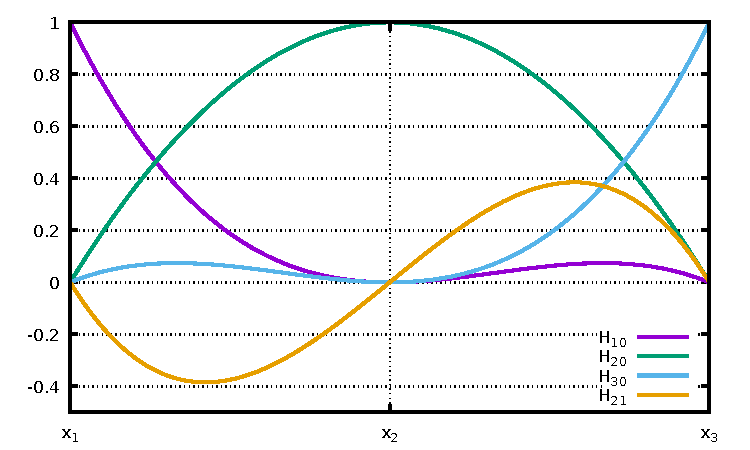
\includegraphics[width=.8\textwidth]{graph/interpolation/simpson}
  \end{center}
\end{frame}

\subsubsection{Gauß-Quadratur}
%\frame{\subtoc}
\frame {\input {blocks/Lemma-quadratur-exakt-max.tex}
  \input {blocks/Satz-gauss-legendre-eindeutig.tex}}
\frame {\input {blocks/Definition-Gauss-Legendre.tex}
  \input {blocks/Satz-gauss-legendre.tex}}
\frame {\input {blocks/Lemma-gauss-legendre-gewichte.tex}
  \input {blocks/Lemma-gauss-legendre-fehler.tex}}

\subsubsection{Richardson-Extrapolation und Romberg-Quadratur}
\frame{\subtoc}
\frame {\input {blocks/Definition-richardson-extrapolation.tex}}
\frame {\input {blocks/Definition-Romberg-quadratur.tex}}
\frame {\input {blocks/Algorithmus-romberg.tex}}
\frame {\input {blocks/Aufgabe-romberg.tex}}

\section{Iterationsverfahren}
\frame{\sectoc}
\frame {\input {blocks/Definition-heron.tex}
\pause \input {blocks/Algorithmus-heron.tex}}
\frame {\input {blocks/Beispiel-heron.tex}}
\subsection{Grundlagen}
\frame{\subtoc}

\subsubsection{Vektor- und Matrixnormen}
\frame {\input {blocks/Definition-norm.tex}}
\frame {\input {blocks/Definition-norm-aequivalenz.tex}}
\frame {\input {blocks/Definition-rn-konvergenz.tex}}
\frame {\input {blocks/Lemma-norm-aequivalenz.tex}}
\frame {\input {blocks/Satz-norm-aequivalenz.tex}}
\frame {\input {blocks/Lemma-norm-aequivalent-konvergenz.tex}}
\frame {\input {blocks/Aufgabe-konvergenz-aequivalenz.tex}}
\frame {\input {blocks/Definition-matrix-norm.tex}}
\frame {\input {blocks/Lemma-operator-norm.tex}}
\frame {\input {blocks/Beispiel-Zeilensummen.tex}}

\frame {\input {blocks/Definition-eigenwert.tex}
  \input {blocks/Lemma-ew-norm.tex}}
\frame {\input {blocks/Satz-onb-ev.tex}
  \input {blocks/Satz-spektralnorm.tex}}
\frame {\input {blocks/Definition-pos-def.tex}
  \input {blocks/Satz-spd.tex}}
\frame {\input {blocks/Definition-matrix-kondition.tex}}

\subsubsection{Fixpunktiterationen}
\frame {\input {blocks/Definition-iteration.tex}}
\frame {\input {blocks/Definition-iteration-ordnung.tex}}
\frame {\input {blocks/Definition-kontraktion.tex}}
\frame {\input {blocks/Satz-bfs.tex}}
\frame {\input {blocks/Satz-lokale-konvergenz.tex}}
\frame {\input {blocks/Satz-optimize-solve.tex}}

\subsection{Das Newton-Verfahren}
\frame{\subtoc}
\frame {\input {blocks/Definition-newton-verfahren.tex}}
\frame {\input {blocks/Algorithmus-newton.tex}}
\frame {\input {blocks/Lemma-newton-1.tex}}
\frame {\input {blocks/Satz-newton-konvergenz.tex}}

\subsection{Abstiegsverfahren und Globalisierung}
\frame{\subtoc}

\frame {\input {blocks/Definition-anstiegskegel.tex}}
\frame {\input {blocks/Lemma-abstieg-reduktion.tex}}
\frame {\input {blocks/Definition-abstiegsverfahren.tex}}
\frame {\input {blocks/Beispiel-steepest-descent.tex}}
\frame {\input {blocks/Satz-abstieg-haeufung.tex}}
\frame {\input {blocks/Korollar-abstieg-haeufung.tex}}


\frame {\input {blocks/Lemma-newton-abstieg.tex}
  \input {blocks/Korollar-newton-abstieg.tex}}
\frame {\input {blocks/Definition-newton-stepsize.tex}}
\frame {\input {blocks/Algorithmus-newton-stepsize.tex}}

\section{Lineare Gleichungssysteme}
\subsection{Grundlagen}
\frame{\sectoc}

\frame {\input {blocks/Satz-lgs-loesbar.tex}}

% \frame {\input {blocks/Definition-eigenwert.tex}}
% \frame {\input {blocks/Lemma-ew-norm.tex}}
% \frame {\input {blocks/Satz-onb-ev.tex}}
% \frame {\input {blocks/Satz-spektralnorm.tex}}
% \frame {\input {blocks/Definition-pos-def.tex}}
% \frame {\input {blocks/Satz-spd.tex}}

\subsection{Konditionierung der Lösung}
\frame {\input {blocks/Definition-aufgabe-loesung.tex}}
\frame {\input {blocks/Lemma-gestoert-invertierbar.tex}}
\frame {\input {blocks/Satz-kondition-lgs.tex}}

\subsection{Die LR-Zerlegung}
\frame{\subtoc}
%\frame {\input {blocks/Notation-quadratische-matrizen.tex}}
\frame {\input {blocks/Definition-dreiecksmatrix.tex}
\input {blocks/Satz-dreieck-gruppe.tex}
\input {blocks/Korollar-dreieck-inverse.tex}}
\frame {\input {blocks/Algorithmus-vorwaerts-rueckwaerts.tex}}
\frame {\input {blocks/Definition-frobenius-matrix.tex}}
\frame {\input {blocks/Lemma-frobenius-matrix.tex}}
\frame {\input {blocks/Lemma-elimination-1.tex}}
\frame {\input {blocks/Satz-elimination-2.tex}}
\frame {\input {blocks/Algorithmus-lr.tex}}
\frame {\input {blocks/Algorithmus-for-back.tex}}
\frame {\input {blocks/Lemma-aufwand-LR.tex}}
\frame {\input {blocks/Satz-existenz-LR.tex}}
\frame {\input {blocks/Definition-spalten-pivot.tex}}
\frame {\input {blocks/Lemma-spalten-pivot.tex}}
\frame {\input {blocks/Lemma-l-p-vertauschung.tex}}
\frame {\input {blocks/Satz-lr-pivot.tex}}
\frame {\input {blocks/Notation-abs-matrix.tex}}
\frame {\input {blocks/Lemma-rundung-lr-1.tex}}
\frame {\input {blocks/Lemma-rundung-vor-rueck.tex}}
\frame {\input {blocks/Satz-rundung-lr-2.tex}}
\frame {\input {blocks/Definition-nachiteration.tex}}
\frame {\input {blocks/Aufgabe-nachiteration-kontraktion.tex}}

\subsection{Die QR-Zerlegung}
\frame{\subtoc}
\frame {\input {blocks/Definition-ortho-matrix.tex}
  \input {blocks/Satz-ortho-matrix.tex}
  \input {blocks/Lemma-qr-norm.tex}}
\frame {\input {blocks/Definition-qr.tex}}
\frame {\input {blocks/Lemma-qr-spalten.tex}}
\frame {\input {blocks/Satz-qr.tex}}
\frame {\input {blocks/Notation-dyadisch.tex}}
\frame {\input {blocks/Lemma-matrix-reflexion.tex}}
\frame {\input {blocks/Lemma-householder-konstruktion.tex}}
\frame {\input {blocks/Algorithmus-householder-1.tex}}
\frame {\input {blocks/Definition-householder-qr.tex}}
\frame {\input {blocks/Lemma-householder-qr.tex}}
\frame {\input {blocks/Lemma-householder-aufwand.tex}}
\frame {\input {blocks/Algorithmus-householder-2.tex}}
\frame {\input {blocks/Lemma-householder-loesung.tex}}
\frame {\input {blocks/Algorithmus-householder-3.tex}}
\frame {\input {blocks/Definition-givens.tex}}
\frame {\input {blocks/Lemma-givens-berechnung.tex}}
\frame {\input {blocks/Lemma-qr-givens.tex}}
\frame {\input {blocks/Algorithmus-givens-2.tex}}
\frame {\input {blocks/Aufgabe-givens-hessenberg.tex}}
\frame {\input {blocks/Lemma-qr-givens-aufwand.tex}}

\subsection{Lineare Ausgleichsrechnung}
\frame{\subtoc}
\frame {\input {blocks/Satz-normalengleichungen.tex}}
\frame {\input {blocks/Definition-condition-rectangular.tex}}
\frame {\input {blocks/Lemma-condition-squared.tex}}
\frame {\input {blocks/Lemma-qr-rectangular.tex}}
\frame {\input {blocks/Satz-qr-normal.tex}}


\subsection{Singulärwertzerlegung und Pseudoinverse}
\frame{\subtoc}

\frame {\input {blocks/Notation-diag.tex}}
\frame {\input {blocks/Definition-svd.tex}}
\frame {\input {blocks/Satz-svd.tex}}
\frame {\input {blocks/Lemma-svd-eigenschaften.tex}}
\frame {\input {blocks/Satz-minimalloesung.tex}}
\frame {\input {blocks/Definition-pseudoinverse.tex}}
\frame {\input {blocks/Satz-penrose.tex}}
\frame {\input {blocks/Definition-epsilon-rang.tex}}
\frame {\input {blocks/Satz-rang-approximation.tex}}
\frame {\input {blocks/Korollar-epsilon-rang.tex}}


\section{Bibliography}
\frame{\bibliographystyle{alpha}
\bibliography{all}}

%\frame {\input {blocks/Satz-trigonometrische-interpolation.tex}}

\end{document}

%%% Local Variables:
%%% mode: latex
%%% TeX-master: t
%%% End:
